\documentclass[a4paper,3cm]{report}
\usepackage{geometry}
\geometry{margin=3cm}
\usepackage[T1]{fontenc}
\usepackage[utf8]{inputenc}
\usepackage[francais]{babel}
\usepackage{amssymb}
\usepackage{mathtools}
\usepackage{graphicx}
\usepackage{color}
\usepackage[dvipsnames]{xcolor}
\usepackage{float}

\definecolor{lgray}{gray}{0.70}
\newcommand\quadri[1]{\noindent
\begin{figure}[H]
\centering
\medbreak
\textcolor{lgray}{
	\setlength\unitlength{5mm}
	\begin{picture}(29,#1)\multiput(0,0)(1,0){30}{\line(0,1){#1}}\put(0,0){\line(1,0){29}}\multiput(0,1)(0,1){#1}{\line(1,0){29}}
	\end{picture}}
\smallbreak
\end{figure}
}


\newcommand\quadribis[2]{%\begin{center}
\begin{figure}[H]
\setlength\unitlength{5mm}
\begin{minipage}{#1\unitlength}\smallbreak\textcolor{gray}{\begin{picture}(#1,#2)
\line(0,1){#2}
\multiput(1,0)(1,0){#1}{\line(0,1){#2}}
\put(0,0){\line(1,0){#1}}
\multiput(0,1)(0,1){#2}{\line(1,0){#1}}
\end{picture}}%\medbreak
\end{minipage}
\end{figure}
%\end{center}
}

\title{PS23 : Ondes et électromagnétisme}
\author{D'après un cours de\\
P. Lanceleur et E. Perrey-Debain\\\\
Retranscrit par\\
H. Lefebvre}

\date{2016}

\begin{document}
\maketitle
\tableofcontents

%PREMIERE PARTIE (PS95)
\part{Electromagnétisme}

\chapter{Electrostatique}
%TEST : \quadribis{4}{5}
L'électrostatique est le domaine de la physique qui étudie les phénomènes créés par des charges électriques statiques. Depuis l'antiquité, il est connu que certains materiaux (dont l'ambre) attirent des objets de petites tailles après avoir été frottés. Le mot grec pour "ambre" est elek-tron.

\section{Structure de la matière}

La vision moderne de la matière décrit celle-ci comme étant constituée d'atomes. Ceux-ci sont eux-même composés d'un noyau (1981, Rutherford) autour duquel "gravite" une sorte de nuage composé d'électrons et portant l'essentiel de la masse. Ces electrons se repoussent les uns les autres mais restent confinés autour du noyau car celui-ci possède une charge positive qui les attire. On attribue cette charge positive à des particules appelés protons. Il existe un autre type de particule, les neutrons, portant une charge électrique nulle. \\\\
Dans le tableau de Mandeliev, tout élement $X$ est representé par la notation \[ X^A_Z \] où $A$ est le nombre de masse (nombre total de nucléon) et $Z$ le numéro atomique (nombre de protons). La charge électrique nucléaire totale est donc
\[ Q=+Ze \]
Et le cortège électrique possède une charge \[Q=-Ze\]
Ce qui assure la neutralité de l'atome. \\\\
\noindent \textbf{Numérique} : Voici quelques données numériques :
\[
\begin{array}{ll}
\textrm{Electron} & 
\left\{
\begin{array}{l}
Q_e=-e=-1.602\times 10^{-19} \textrm{ C} \\
m_e=9.109\times 10^{-31}\textrm{ kg}
\end{array}
\right. \\
\textrm{Proton} & 
\left\{
\begin{array}{l}
Q_p=+e=1.602\times 10^{-19} \textrm{ C} \\
m_p=1.672\times 10^{-27} \textrm{ kg}
\end{array}
\right.
\\
\textrm{Neutron} & 
\left\{
\begin{array}{l}
Q_n=0 \\
m_n=1.674 \times 10^{-27} \textrm{ kg}
\end{array}
\right.
\\
\end{array}
\]
A l'heure actuelle, l'univers est descriptible à l'aide des 4 forces fondamentales :
\begin{itemize}
\item Force nucléaire faible (radioactivité)
\item Force nucléaire forte (cohésion du noyau)
\item Force électromagnétique (cohésion de l'atome)
\item Force gravitationnelle (cohésion des corps astro-physiques)
\end{itemize}
Un matériau est ainsi constitué d'un grand nombre de charges électriques, mais celles-ci sont toutes compensées. Des charges en excés ou en manque, non compensées, sont responsables des effets électriques. \\\\
\noindent\textbf{Conducteur parfait} : Un matériau est dit conducteur parfait si lorsqu'il devient electrisé, les porteurs de charges non compensées peuvent se déplacer librement dans tout le volume occupé par le materiau. (exemple : électrolyse, conducteur ohmique)\\\\
\noindent\textbf{Isolant parfait} : Un matériau est dit isolant (ou diélectrique) parfait si les porteurs de charges restent "immobiles".

\section{Forces, champs et potentielles}
\subsection{Force de Coulomb}

\par Charles Auguste Coulomb (1736-1806) a effectué une série de mesures qui lui ont permis de déterminer avec un certain degré de précision les propriétés de la force électrostatiques. La force est radiale et proportionnelle au produit des charges et varie comme l'inverse du carré de la distance entre les charges.
\quadri{5}
\noindent\textbf{Définition} : La force exercée par une charge ponctuelle $q_1$ sur une autre charge $q_2$ est :
\[ \vec{F}_{1/2}=\frac{1}{4\pi\varepsilon_0}\frac{q_1q_2}{r_{1,2}^2}\vec{u}_{1,2} \]
Où $k=\frac{1}{4\pi\varepsilon_0}=9\times 10^9 \textrm{ Nm}^2\textrm{C}^{-2}$, $\varepsilon$ la permitivité du vide (en Farad par mètre) et où $\vec{u}_{1,2}$ est vecteur unitaire allant de $1$ vers $2$. (Attention, dans un milieu différent du vide, la constante de permitivité doit être adapté)
\\\\
\noindent\emph{Remarque} : Pour un électron, la force de gravité est hautement négligeable par rapport à la force électromagnétique, en effet \[ \frac{F_e}{F_g}=\frac{e^2}{4\pi\varepsilon_0 r^2}\left(\frac{Gm_e^2}{r^2}\right)^{-1}=4\times 10^{42} \]

\subsection{Champ électrostatique}

Pour une charge ponctuelle, on peut remarquer que $\frac{\vec{F}_{1/2}}{q_2}$ ne dépend que de la charge $q_1$ et de la distance $r_{1,2}$. On appelle cette quantité vectorielle "champ électrique"\\\\
\noindent\textbf{Champ électrostatique} : Une charge $q$ en un point $P$ de l'espace, crée en un point $M$ de l'espace un champ électrostatique $\vec{E}(M)$ en V/m telle que :
\[ \vec{E}(M)=\frac{1}{4\pi \varepsilon_0}\frac{q}{r^2}\vec{u} \]
\noindent\textbf{Champ créé par un ensemble de charge} : D'après le principe de superposition, le champ résultant en un point $M$ est égale à la somme de tous les champs électriques de chacunes des charges $q_i$ ($i=1...n$) placés en $P_i$. De sorte qu'en notant $\vec{r}_i=\vec{P_iM}$ et $\vec{u}_i=\vec{r}_i/\mid\mid\vec{r}_i\mid\mid$
\[ \vec{E}(M)=\frac{1}{4\pi \varepsilon_0}\sum_{i=1}^n\frac{q_i}{r_i^2}\vec{u}_i \]
En pratique, cette expression n'est que rarement utilisée puisque nous sommes amenés à considérer un nombre gigantesque de particules. Il est donc plus habile d'utiliser des distributions continues de charge. Il s'agit d'une approximation, permettant de remplacer une somme discrète presqu'infinie par une somme continu :
\[ \vec{E}(M)=\int_{dist}\frac{dq(P)}{4\pi\varepsilon_0 r^2}\vec{u} \]
Avec $dq(P)$ la charge en $P$ et $\vec{r}=\vec{PM}$
\\\\\noindent\textbf{Densités} : Pour caractériser la distribution de charges sur un volume, on introduit les densités de charges suivantes \\
\begin{center}
\begin{tabular}{|c|c|c|}
\hline
Densité linéique & Densité surfacique & Densité volumique  \\
\hline
$\lambda=\frac{dq}{dl}$ & $\sigma=\frac{dq}{dS}$ & $\rho=\frac{dq}{dV}$ \\
\hline
$\vec{E}(M)=\frac{1}{4\pi\varepsilon_0}\int_C\frac{\lambda}{r^2}\vec{u}dl$ & 
$\vec{E}(M)=\frac{1}{4\pi\varepsilon_0}\iint_\Sigma\frac{\lambda}{r^2}\vec{u}dl$ &
$\vec{E}(M)=\frac{1}{4\pi\varepsilon_0}\iiint_V\frac{\lambda}{r^2}\vec{u}dl$ \\
\hline
\end{tabular}
\end{center}
\quadri{6}

\subsection{Application}
Ces phénomènes électrostatiques sont utilisés par exemple pour dévier une particule de charge $q$. En effet, d'après le principe fondamentale de la dynamique : 
\[ \vec{F}=m\frac{d\vec{v}}{dt}=q\vec{E}\Rightarrow
\left\{
\begin{array}{l}
x=v_0t\\
y=\frac{1}{2} \frac{qE}{m}t^2
\end{array}
\right. \Rightarrow y=\frac{qE}{2mv_0^2}x^2 \]
\quadri{10}

\section{Théorème de Gauss}
\subsection{Notion d'angle solide}
La notion d'angle solide est l'extension naturelle dans l'espace de l'angle défini sur un plan. \\\\
\noindent\textbf{Définition} : L'angle solide élementaire $d\Omega$, délimité par un cône coupant un élement de surface $dS'$ à distance $r$ de son sommet $O$ vaut :
\[ d\Omega=\frac{dS'}{r^2} \]
\quadri{7}
D'une façon génerale, le cône peut intercepter une surface quelconque $dS$ dont la normale $\vec{n}$ fait un angle $\theta$ avec le vecteur unitaire $\vec{u}$. On a alors bien sûr $\vec{n}.\vec{u}=\cos\theta$ et on peut considérer que $dS'=dS\cos\theta$, d'où
\[ d\Omega=\frac{dS'}{r^2}=\frac{dS\cos\theta}{r^2}=\frac{dS\vec{n}.\vec{u}}{r^2} \]

\subsection{Flux d'un champ électrostatique}

On considère une charge ponctuelle $q$ en $O$. Le flux du champ $\vec{E}$ dû à $q$ à travers une surface élementaire $\vec{dS}=dS\vec{n}$ est
\[ d\Phi=\vec{E}.\vec{dS}=\vec{E}.\vec{n}dS=\frac{1}{4\pi\varepsilon_0}\frac{q}{r^2}\vec{u}.\vec{n}dS=\frac{q}{4\pi\varepsilon_0}d\Omega \]

\subsection{Théorème de Gauss}

Que se passe-t-il si on s'intéresse au flux total à travers une surface fermée ?
\quadri{11}
\noindent\textbf{Bilan du flux sur le cône $d\Omega$} : Comme la surface considérée est fermée, le nombre de traversées du cône est toujours impair (cf. ci-dessus). Ainsi, pour une traversée : \[ d\Phi=\frac{qd\Omega}{4\pi\varepsilon_0} \]
Pour trois traversées : \[ d\Phi=d\Phi_1+d\Phi_2+d\Phi_3=\frac{q}{4\pi\varepsilon_0}(d\Omega-d\Omega+d\Omega)=\frac{qd\Omega}{4\pi\varepsilon_0} \]
Ceci se vérifie encore pour un nombre supérieur de traversées du cône. Et, en intégrant selon toutes les distances, on trouve :
\[ \Phi=\iint_\Sigma d\Phi=\iint_\Sigma\frac{qd\Omega}{4\pi\varepsilon_0}=\frac{q}{\varepsilon_0} \]
Ce résultat se généralise encore pour un nombre quelconque de charges, c'est le théorème de Gauss.\\\\
\noindent\textbf{Théorème de Gauss} : \[ \Phi=\iint_\Sigma\vec{E}.\vec{n} dS=\frac{Q_{int}}{\varepsilon_0}\]

\subsection{Equation de Maxwell-Gauss}

Le théorème de Gauss-Ostrogradski (MT22) nous permet d'affirmer que 
\[ \iint_\Sigma\vec{E}.\vec{n}dS=\iiint_V\textrm{div }\vec{E}dV \]
Or, dans le cas d'une distribution volumique de charge, on a
\[ \iint_\Sigma\vec{E}.\vec{n}dS=\iiint_V\frac{\rho}{\varepsilon_0}dV \]
Ce qui nous permet de déduire la première des équations de Maxwell :
\[ \textrm{div }\vec{E}=\frac{\rho}{\varepsilon_0} \]


\section{Energies et travail}
\subsection{Cas d'une charge ponctuelle}
Prenons une particule "test" de charge $q_t$ placée dans un champ électrostatique $\vec{E}$ créé par une autre charge $q$ placée au point $P$. Pour déplacer la charge $q_t$ du point $A$ au point $B$, un opérateur doit fournir une force qui s'oppose à la force de Coulomb. Si ce déplacement est fait suffisamment lentement, $\vec{F}=-q_t\vec{E}$ et le travail fourni par l'opérateur est donné par \[ W_A^B=\int_A^B\vec{F}.\vec{dl}=-q_t\int_A^B\vec{E}.\vec{dl}=\int_A^B\frac{q}{4\pi\varepsilon_0}\frac{\vec{u}.\vec{dl}}{r^2}=-q_t\int_A^B\frac{q}{4\pi\varepsilon_0 r^2}\cos\theta dl=-q_t\int_A^B\frac{qdr}{4\pi\varepsilon_0 r^2} \]
Par ailleurs, si on note $V(M)$ le potentiel électrostatique tel que \[ V(M)=\frac{q}{4\pi\varepsilon_0 r} \]
On trouve que \[ W_A^B = q_t(V(B)-V(A)) \]
\quadri{10}
\emph{Remarque} : La force électrostatique est conservative\\\\
\noindent\textbf{Energie potentielle} : L'energie potentielle d'une particule chargée $q_t$ placée dans un champ électrostatique est égale au travail qu'il faut fournir pour amener de façon quasi-statique cette particule de l'infini à sa position actuelle.
\[ U=W_\infty^M=q_t(V(M)-V(\infty))=q_tV(M) \textrm{ Car, par convention : }V(\infty)=0 \]\\
\noindent\textbf{Relation entre $\vec{E}(M)$ et $U(M)$} : Considérons deux points très proche $M$ et $M'$. On a $\vec{MM'}=\vec{dl}$. On a alors d'une part
\[ dV=V(M')-V(M)=-\int_M^{M'}\vec{E}.\vec{dl}=-\vec{E}.\vec{dl} \]
Et d'autre part
\[ V=V(x,y,z)=\frac{\partial U}{\partial x}dx+\frac{\partial U}{\partial y}dy+\frac{\partial U}{\partial z}dz=\vec{\textrm{grad }}V.\vec{dl} \]
D'où  l'égalité suivante :
\[ \vec{E}=-\vec{\textrm{grad }}V \]

\subsection{Cas d'une distribution de charge}

Fixons une particule de charge $q_1$. Le travail nécessaire pour amener une charge $q_2$ est \[ U_2=q_2V_{12}=\frac{1}{4\pi\varepsilon_0}\frac{q_1q_2}{r_{12}} \]
De même, le travail pour amener une troisième charge $q_3$ est \[ U_3=q_3(V_{13}+V_{23})=\frac{q_1q_3}{r_{13}}+\frac{q_2q_3}{r_{23}} \]
Enfin, pour $n$ charges $q_i$, on trouve
\[ U=U_1+U_2+...+U_n=\frac{1}{4\pi\varepsilon_0}\sum_{i=1}^nq_i\sum_{j<i}\frac{q_j}{r_{ij}}=\frac{1}{2}\sum_{i=1}^nq_iV_i \] Où $V_i$ est le potentiel en $i$ dû aux autres charges. \\\\
\noindent Ce résultat se géneralise pour une distribution de charge par
\[ U=\frac{1}{2}\int_{dist}dq(M)V(M) \textrm{ où }V(M)=\frac{1}{4\pi\varepsilon_0}\int_{dist}\frac{dq}{r} \]
\emph{Remarque} : $V$ est exprimé en Volt (V) alors que $V$ est exprimé en électron-volt (eV). $1 $eV$=1.6\times 10^{-19}$ J.

\subsection{Surfaces équipotentielles}

\noindent\textbf{Définition} : La surface équipotentielle est telle que le potentiel $V$ est constant en tout point de celle-ci.
\[V(x,y,z)=\textrm{cte}\Rightarrow dV=\vec{\textrm{grad }}V.\vec{dl}=0\Rightarrow\vec{E}.\vec{dl}=0\]


\chapter{Conducteur en équilibre}
\section{Conducteurs isolés}

\noindent\textbf{Définition} : L'équilibre électrostatique d'un conducteur est atteint lorsqu'une charge électrique ne se déplace plus à l'intérieur du conducteur. Cela entraine nécessairement que :
\begin{itemize}
\item Le champ électrostatique total est nul dans le conducteur. (i.e. $\vec{E}=0$ et donc $V=\textrm{cte}$)
\item Les charges sont localisées à la surface.\\
\end{itemize}
\noindent\textbf{Théorème} : Le champ électrostatique à proximité immédiate d'un conducteur de densité surfacique $\sigma$ vaut :
\[ \vec{E}=\frac{\sigma}{\varepsilon_0}\vec{n} \]

\section{Influence électrostatique}
\quadri{20}

\section{Application : Condensateur}
\quadri{30}


\chapter{Magnétostatique}
\section{Introduction}

La magnétostatique est l'étude du magnétisme dans les situations où le champ magnétique ne dépend pas du temps. Il existe deux sources de champs magnétiques : le courant électrique et la matière aimantée. L'analyse du champ magnétique commence avec l'experience de Orsted (1820, 40 ans après Coulomb) : il place un fil conducteur au dessus d'une boussole par hasard et y fait passer un courant. 

\section{Champ magnétique}
\subsection{Champ créé par une charge en mouvement}

Le champ magnétique créé en un point $M$ par une particule $q$ située en $P$ et animée d'une vitesse $\vec{v}$ est 
\[ \vec{B}(M)=\frac{\mu_0}{4\pi}\frac{q\vec{v}\land\vec{u}}{r^2} \]
\emph{Remarque} : L'unité du champ magnétique est le Tesla. $\mu_0$ est la perméabilité du vide et vaut $\mu_0=4\pi\times 10^{-7}$ H.m$^{-1}$
\subsection{Champ créé par un ensemble de charges}
Le principe de superposition nous permet de déduire que, pour un ensemble de charge, le champ magnétique vaut :
\[ \vec{B}(M)=\frac{\mu_0}{4\pi}\sum_{i=0}^n\frac{q_i\vec{v_i}\land\vec{u_i}}{r_i^1} \]
Et pour une distribution de charge continu :
\[ \vec{B}(M)=\frac{\mu_0}{4\pi}\int_\nu\frac{dq\vec{v}\land\vec{u}}{r^1} \]

\subsection{Champ créé par un circuit électrique}

Considérons un conducteur métallique, les porteurs de charge sont les électrons et on a 
\[ dq\vec{v}=nq\vec{v}d\nu=\vec{j}d\nu\vec{v} \]
Avec $n$ la densité de porteur de charge, $\vec{j}$ le vecteur densité et $\nu$ le volume ($d\nu=Sdl$). On a évidemment $\vec{dl}=\vec{v}dt$. \\\\
\noindent On s'intéresse ici à une partie infinitésimalle d'un circuit. Calculons le champ magnétique élementaire :
\[ d\vec{B}=\frac{\mu_0}{4\pi}\left[\iint_S\vec{j}.\vec{dS}\right]\vec{dl}\land\vec{u} \]
Or, \[ \iint_S\vec{j}.\vec{dS}=I\vec{dl} \]
\quadri{10}
Avec $I$ le courant. On trouve la fameuse loi de Biot et Savart :
\[ \vec{B}(M)=\frac{\mu_0}{4\pi}\int_C\frac{I\vec{dl}\land\vec{u}}{r^2} \]
\emph{Remarque} : Le courant électrique est donnée par $I=nevS$ avec $n$ la densité de porteur de charge, $e$ la charge d'un électron, $v$ la vitesse moyenne de dérive et $S$ la section du fil considéré.

\section{Théorème d'Ampère}
\subsection{Théorème d'Ampère}

Considérons tout d'abord un fil de longueur infinie, on a notamment :
\[ \vec{OM}=r\vec{e_r}+z\vec{e_z} \textrm{ et donc } d\vec{OM}=\vec{dl}=dr\vec{e_r}+rd\theta\vec{e_\theta}+dz\vec{e_z} \]
Le calcul de la circulation du champ magnétique selon une courbe fermée est alors assez remarquable :
\[ C_\Gamma=\oint_\Gamma\vec{B}.\vec{dl}=\mu_0I\oint_\theta\frac{d\theta}{2\pi} \]
Deux cas sont alors possibles, soit $\Gamma$ est une courbe qui n'enlace pas le fil, auquel cas $\oint_\theta\frac{d\theta}{2\pi}=0$. Soit $\Gamma$ enlace le fil et alors $\oint_\Gamma\vec{B}.\vec{dl}=\mu_0I$ (car alors $\oint_\theta\frac{d\theta}{2\pi}=1$). Ce résultat se généralise par le théorème d'Ampère.\\\\

\noindent\textbf{Théorème d'Ampère} : La circulation de $\vec B$ le long d'une courbe orientée, fermée, appelée alors contour d'Ampère, est égale à $\mu_0$ fois la somme algébrique des courants qui traversent la surface $S_\Gamma$ délimité par $\Gamma$. Ou encore :
\[ \oint_\Gamma\vec{B}.\vec{dl}=\mu_0I_{Total} \]
\quadri{5}
\emph{Remarque} : Le choix du sens de la circulation est arbitraire. 



\subsection{Equation de Maxwell-Thomson}

\noindent\emph{Rappel} : Pour une charge placée en $O$ animée d'une vitesse $\vec{v}=v\vec{e_z}$, on trouve que 
\[ \vec{B}(M)=\frac{\mu_0 q\vec{v}\land\vec{e_\theta}}{(r^2+z^2)^{3/2}} \]
\quadri{7}
\noindent\textbf{Equation de Maxwell-Thomson} : On a toujours : \[ \textrm{div }\vec{B}=0 \]

\subsection{Equation de Maxwell-Ampère}

On vient d'établir que \[ \oint_\Gamma\vec{B}.\vec{dl}=\mu_0\iint_{S_\Gamma}\vec{j}.\vec{n}dS \]
Or, la relation suivante est aussi verifiée (MT22) :
\[ \iint_{S_\Gamma}\vec{\textrm{rot }}\vec{B}.\vec{dS}=\oint_\Gamma \vec{B}.\vec{dl} \]
Ce qui nous permet de déduire
\[ \vec{\textrm{rot }}\vec{B}=\mu_0\vec{j} \]
\emph{Remarque importante} : Ceci est vrai uniquement si $\vec{j}$ est constant

\section{Actions magnétiques}
\subsection{Force magnétique subit par une particule chargée}

\noindent\textbf{Force de Lorentz} : La force totale, électrique et magnétique, subie par une particule de charge $q$ et de vitese $\vec{v}$ (mesuré dans un réferentielle galiléen) est \[ \vec{F_L}=q(\vec{E}+\vec{v}\land\vec{B}) \]
\emph{Remarque} : La composante magnétique ne fournit pas de travail.\\\\
\noindent Etudions la trajectoire d'une particule chargée en présence d'un champ magnétique. On considère une particule de masse $m$ et de charge $q$. A $t=0$, $\vec{v}(t)=\vec{v_0}$. Le principe fondamental de la dynamique nous donne
\[ m\frac{d\vec{v}}{dt}=q\vec{v}\land\vec{B} \]
\emph{Rappel PS21} : \[\frac{d\vec{v}}{dt}=a_T\vec{T}+\frac{v^2}{R}\vec{N}\]
Or, on a clairement $q\vec{v}\land\vec{B}\perp\vec{T}$, ce qui implique que
\[ a_T=\frac{dv}{dt}=0 \textrm{ et donc }v=v_0=\textrm{cte} \]
D'où finalement
\[ m\frac{v_0^2}{R}=\mid qv_0B\mid \Rightarrow R=\mid\frac{mv_0}{qB}\mid=\textrm{cte} \]
\quadri{5}

\subsection{Force magnétique subit par un circuit}

\noindent\textbf{Force de Laplace} : 
\quadri{7}
La force magnétique s'exerçant sur un élement de volume $d\nu=S\vec{dl}$ s'écrit 
\[ d\vec{F}=dq\vec{v}\land\vec{B}=\left[\iint_\Sigma\vec{j}dS\right]\vec{dl}\land\vec{B}=I \vec{dl}\land\vec{B}\]
Ainsi, la force totale subit par un fil, appelé force de Laplace est :
\[ \vec{F}=I\int_{circuit}\vec{dl}\land\vec{B} \]
\emph{Remarque} : A partir de la force de Lorentz, qui est une force microscopique agissant sur des particules individuelles, nous avons obtenu une force macroscopique agissant sur un solide. La force de Laplace est capable de déplacer le solide et donc d'exercer un travail non nul. Il faut interpréter cette force comme la résultante de l'action des particules sur le réseau cristallin. En fait, cela se traduit par la présence d'un champ électrostatique : la champ de Hall (cf. Wikipedia).\\\\
\noindent\emph{Remarque 2} : C'est par la mesure de cette force qu'a été défini l'Ampère. L'Ampère est l'intensité du couant dans deux fils situés à $1$ m et produisant une attraction réciproque $F=2\times 10^{-7}$ N.




\chapter{Electrocinétique et induction}
\section{Electrocinétique}
\subsection{Loi d'Ohm}

\emph{Rappel} : \quadri{5} Le courant traversant un tronçon de circuit de section $S$ est \[ I=\frac{dQ}{dt}=\iint_S\vec{j}.\vec{n}dS \]
Dans la plupart des conducteurs, on observe une proportionalité entre la densité de courant ($\vec{j}$) et le champ électromoteur : $\vec{E}_m=\frac{\vec{F}}{q}$ (où $\vec{F}$ est la force responsable du mouvement des électrons)\\\\
\noindent\textbf{Loi d'ohm} : \[ \vec{j}=\gamma\vec{E}_m \]
Où $\gamma$ est appelé conductivité et $\eta=\gamma^{-1}$ est appelé la résistivité.\\\\
\noindent On défnit alors la résistance d'un conducteur de section $S$ et de longueur $L$ par
\[ R=\frac{\int_L\vec{E}_m.\vec{dl}}{I=\iint_S\vec{j}.\vec{n}dS}=\frac{\int_L\vec{E}_m.\vec{dl}}{\iint_S\gamma\vec{E}_m.\vec{n}dS} \]
\emph{Remarque} : Si $E_m$ est constant, alors $R=\frac{\eta L}{S}$\\\\
\noindent\emph{Remarque 2} : Si  le champ électromoteur est d'origine électrostatique pure, alors $\vec{E}_m=-\vec{\textrm{grad }}V$ et donc : 
\[ R=\frac{\int_L\vec{E}_m.\vec{dl}}{I}=\frac{-\int_L\vec{\textrm{grad }}V.\vec{dl}}{I}=\frac{V_A-V_B}{I} \]

\subsection{Conservation de la charge}
Considérons une surface $S$ délimité par un volume $\nu$. Alors,
\[ \frac{dQ}{dt}=\iiint_\nu\frac{\partial \rho}{\partial \rho}d\nu=-\iint_S\vec{j}.\vec{n}dS=\iint_\nu\textrm{div }\vec{j}d\nu \]
D'où finalement : 
\[ \frac{\partial\rho}{\partial t}+\textrm{div }\vec{j}=0 \]

\section{Induction}
\subsection{Expérience de Faraday}
\quadri{13}
\noindent\textbf{Loi de Faraday} : La variation temporelle du flux magnétique à travers un circuit fermé y engendre une force électromotrice induite notée $e$ ou $fem$ telle que
\[ e=\oint_C\vec{E}_m.\vec{dl}=-\frac{d\Phi}{dt} \]
Où $\Phi=\iint_S\vec{B}.\vec{n}dS$\\\\
\noindent\textbf{Loi de Lenz} : L'induction produit des effets qui s'opposent aux causes qui lui ont donné naissance.\\
Par exemple, Si $B$ augmente, le circuit $C$  va être telle qu'il va créer un champ $B_2$ qui va s'opposer à l'accroissement de $B$.
\subsection{Equation de Maxwell-Faraday}
Lorsqu'un courant variable circule dans un circuit, un champ magnétique est créé. Dans ce cas précis, la force induite doit être dû à la composante électrique de la force de Lorentz. On a :
\[ e=\oint_C\vec{E}.\vec{dl}=-\frac{d}{dt}\left(\iint_S\vec{B}.\vec{n}dS\right) \]
Or, on a (MT22) :
\[ \oint_C\vec{E}.\vec{dl}=\iint_S\vec{\textrm{rot }}\vec{E}.\vec{n}dl \]
D'où enfin, l'équation  de Maxwell-Faraday
\[ \vec{\textrm{rot }}\vec{E}=-\frac{\partial\vec{B}}{\partial t} \]

\subsection{Auto-induction et induction mutuelle}

Un circuit isolé est parcouru par un courant $I$, ce courant engendre un champ magnétique, et donc un flux
\[ \Phi=\iint_S\vec{B}.\vec{n}dS=\left[\frac{\mu_0}{4\pi}\iint_S\left(\oint_C\frac{\vec{dl}\land\vec{u}}{r^2}\right)\right].I=L.I \]
En notant
\[ L= \frac{\mu_0}{4\pi}\iint_S\left(\oint_C\frac{\vec{dl}\land\vec{u}}{r^2}\right) \]
Enfin, d'après Faraday, la relation bien connue suivante est toujours vérifiée :
\[ e=-L\frac{dI}{dt} \]

\subsection{Retour sur les équations de Maxwell}

\quadri{30}



%DEUXIEME PARTIE (PS96)
\part{Ondes}

\chapter{Equation des ondes et solutions}
\section{Définitions}
\noindent\textbf{Perturbation} : Petite variation d'une quantité physique \\ \\
\textbf{Onde} : Perturbation dynamique de toute quantité physique rendant compte de l'état d'un milieu, susceptible de se propager dans l'espace et le temps.\\ \\
\textbf{Propagation} : Déplacement au cours du temps du phénomène dans un milieu qui "reste immobile" et revient à son état initial après le passage de l'onde. \\ \\
\textbf{Equation d'onde} Si $\varphi$ est une onde, alors :
\[\Delta\varphi(M,t)-\frac{1}{c_0^2}\frac{\partial^2\varphi}{\partial t^2}(M,t)=0, \forall M, t\]\\
\emph{Remarque} : L'équation d'onde traduit bien la définition donnée ci-dessus : $\Delta\varphi$ représente la variation spatiale alors que $\frac{\partial^2\varphi}{\partial t^2}$ représente la variation temporelle du phénomène. Le terme $1/c_0^2$ rend homogène la formule. 
\section{Description}
\quadri{7}
Ici, la perturbation qui a lieu en $t=t_0$ se propage dans le temps. C'est à dire que la "même perturbation" se retrouve à l'instant suivant $t=t_0+\Delta t$.\\ \\
\textbf{Célérité} : En une durée $\Delta t = t-t_0$, l'onde se propage sur une distance $d=x-x_0$. On note alors $c=\frac{x-x_0}{t-t_0}$ la célerité de l'onde qui correspond au déplacement de la perturbation.\\ \\
\emph{Remarque} : Ne pas confondre vitesse et celérité ! En effet, la vitesse est associée à un déplacement de masse alors que la celérité est liée à la propagation d'un phénomène. \\
Ici par exemple, l'onde est transversale et $v=dy/dt$, avec $c>>v$ \\ \\
\textbf{Propagation} : \[ c=\frac{x-x_0}{t-t_0} \Leftrightarrow c(t-t_0) = x-x_0 \Leftrightarrow x-ct=x_0-ct_0 \]
Or $x_0-ct_0$ est constant ! On appelle alors "$x-ct$" le propagateur de l'onde. \\ \\
\textbf{Progression} : On établit facilement le sens de la propagation en fonction du propagateur : 
\begin{itemize}
  \item $x-ct$ : l'onde se propage dans le sens des $x$ croissant (signes différents)
  \item $x+ct$ : l'onde se propage dans le sens des $x$ décroissant (signes identiques)\\
\end{itemize}

\noindent\textbf{Solutions de l'équation} (Proposition) : $\varphi(M,t)=f(x-ct)+g(x+ct)$ est solution de l'équation des ondes. \\
\emph{Preuve} : 
\[
\left \{
  \begin{array}{l}
  \Delta\varphi=\frac{\partial^2(f+g)}{\partial x^2}=f''+g'' \\
  \frac{\partial(f+g)}{\partial t}=-c(f+g)
  \end{array}
\right.
\Rightarrow 
\left \{
  \begin{array}{l}
  \Delta\varphi=\frac{\partial^2(f+g)}{\partial x^2}=f''+g'' \\
  \frac{\partial^2(f+g)}{\partial t^2}=c^2(f''+g'') \\
  \end{array}
\right.
\Rightarrow \Delta\varphi-\frac{1}{c_0^2}\frac{\partial^2\varphi}{\partial t^2}=f''+g''-\frac{1}{c_0^2}(c^2(f''+g''))=0
\]



\chapter{Ondes planes et harmoniques}
\section{Définitions}
\noindent\textbf{Onde plane} : Onde qui ne dépend que d'une seule variable cartésienne \\
\textbf{Onde harmonique} : Onde dont le profil est sinusoïdal ($\sim \cos, \sin$) \\
\\
\textbf{Notation} : Dans tout le cours, on notera \\
\indent $A$ : Amplitude (de la même unité que $\varphi$) \\
\indent $\omega$ : Pulsation (en rad/s) \\
\indent $\delta$ : Déphasage (en rad) \\
\indent $f$ : Fréquence (en Hz)\\
\indent $T$ : Periode temporelle \\\\
\noindent\textbf{Définition mathématique} :
On sait que $\varphi$ est une onde plane harmonique progressive si $\varphi(x,t)=f(x-ct)$ avec $f$ une fonction sinusoïdale.\\
Considérons donc qu'à l'instant $t=0$ une perturbation soit provoquée par une source sinusoïdale. On a alors :
\[\varphi(0,t)=A\cos(\omega t +\delta)\]
Avec, par définition, $\omega=2\pi f$ et $f=T^{-1}$\\
On peut alors écrire : \[\varphi(0,t)=A\cos(2\pi f+\delta)=A\cos(\frac{2\pi t}{T}+\delta)\] 
Or, la perturbation qui a lieu en $t=0$ a lieu également un instant plus tard $t+\Delta t$ en $x$ (phénomène de propagation à la celerité $c$) :
\[\varphi(x,t+\Delta t)=\varphi(0,t)=A\cos(\frac{2\pi t}{T}+\delta)\]
D'où :
\[
\varphi(x,t)=\varphi(0,t-\Delta t)=A\cos(2\pi(\frac{t-\Delta t}{T})+\delta)=A\cos(2\pi(\frac{t}{T}-\frac{c\Delta t}{cT})+\delta)=
A\cos(2\pi(\frac{t}{T}-\frac{x}{cT})+\delta)
\]
En posant $\lambda=cT$ la longueur d'onde, on a :
\[\varphi(x,t)=A\cos(2\pi(\frac{t}{T}-\frac{x}{\lambda}))\]
On pose également $k=\frac{2\pi}{\lambda}=\frac{\omega}{c}$\\
\quadri{8}
\[\forall t,x\in \mathbb{R}, n\in\mathbb{N}, \varphi(x+n\lambda,t)=\varphi(x,t)\]
\quadri{8}
\[\forall t,x\in \mathbb{R}, n\in\mathbb{N}, \varphi(x,t+nT)=\varphi(x,t)\]

\section{Equation d'Helmotz}
Etant donné notre connaissance de la forme général des ondes planes harmoniques, on peut simplifier l'équation d'onde les concernant, en effet :
\[
\left \{
  \begin{array}{ll}
  \Delta\varphi-\frac{1}{c^2}\frac{\partial^2\varphi}{\partial t^2}=0 \\
  \varphi(x,t)=A\cos(\omega t -kx+\delta) \\
  \end{array}
\right.
\Rightarrow
\left \{
  \begin{array}{ll}
  \Delta\varphi-\frac{1}{c^2}\frac{\partial^2\varphi}{\partial t^2}=0 \\
  \frac{\partial\varphi}{\partial t}=-A\omega\sin(\omega t -kx)
  \end{array}
\right.
\Rightarrow
\left \{
  \begin{array}{ll}
  \Delta\varphi-\frac{1}{c^2}\frac{\partial^2\varphi}{\partial t^2}=0 \\
  \frac{\partial^2\varphi}{\partial t^2}=-A\omega^2\cos(\omega t -kx)=-\omega^2\varphi(x,t)
  \end{array}
\right.
\]
On a alors : 
\[ \Delta\varphi+\frac{\omega^2}{c^2}\varphi = 0 \Leftrightarrow \Delta\varphi+k^2\varphi = 0 \]
Cette équation est appelée "équation d'Helmotz".

\section{Direction quelconque}
Jusqu'ici, les ondes se propageaient selon l'axe $\vec{e_x}$. Pour une direction quelconque, on introduit le vecteur d'onde $\vec{k}=k\vec{n}$ où $\vec{n}$ est dans la direction de propagation de l'onde ($\mid\mid\vec{n}\mid\mid=1$).\\
Ceci permet d'écrire pour $\vec{r}=\vec{OM}$ (fixe) : 
\[\varphi(\vec{r},t)=A\cos(\omega t -\vec{k}.\vec{r})\]
On a, par ailleurs, la relation suivante, appelée relation de dispertion : $\vec{k}^2=k^2$

\section{Représentation}

\noindent\textbf{Représentation en 1D} :
\begin{center}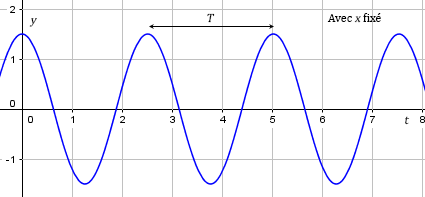
\includegraphics[width=8cm]{img/periode_T.png}\end{center}
\textbf{Représentation en 2D} :
\begin{center}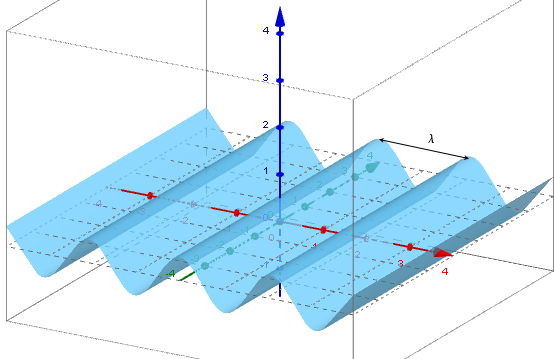
\includegraphics[width=8cm]{img/onde_2D.png}\end{center}
\textbf{Représentation en 3D} :
\begin{center}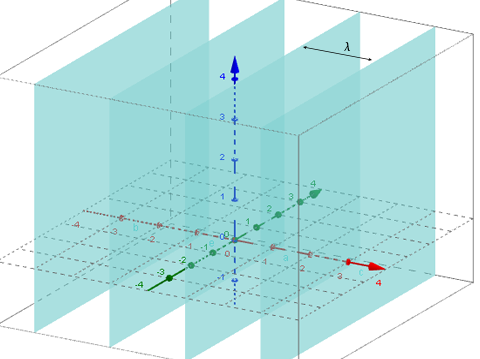
\includegraphics[width=8cm]{img/onde_3D.png}\end{center}

\section{Exemples d'ondes planes harmoniques}

\subsection{Ondes électromagnétiques}

\noindent\textbf{Célérité} : \\
Le champ électromagnétique $\vec{E}$ vérifie l'équation d'onde 
\[\Delta E-\frac{1}{c^2}\frac{\partial^2E}{\partial t^2}=0\]
Pour étudier la propagation des ondes électromagnétiques, on se place en dehors de la source ($\vec{j}=0$ et $\rho=0$). Les équations de Maxwell donnent alors :
\[
\left \{
  \begin{array}{l}
  \textrm{div }\vec{E}=0 \\
  \textrm{div }\vec{B}=0
  \end{array}
\right.
\textrm{ et }
\left \{
  \begin{array}{l}
  \vec{\textrm{rot }}\vec{E}=-\frac{\partial{\vec{B}}}{\partial t} \\
  \vec{\textrm{rot }}\vec{B}=\mu_0\varepsilon_0\frac{\partial\vec{E}}{\partial t}
  \end{array}
\right.
\]
Or : \[\Delta\vec{E}=\vec{\textrm{grad }}\textrm{div }\vec{E}-\vec{\textrm{rot }}\vec{\textrm{rot }}\vec{E}=-\vec{\textrm{rot }}\vec{\textrm{rot }}\vec{E}\] (car $\textrm{div }\vec{E} = 0$)\\
D'autre part : \[\frac{\partial^2\vec{E}}{\partial t^2}=\frac{\partial}{\partial t}(\frac{\partial\vec{E}}{\partial t})=\frac{\partial}{\partial t}(\frac{1}{\mu_0\varepsilon_0}\vec{\textrm{rot }}\vec{B})=\frac{1}{\mu_0\varepsilon_0}\vec{\textrm{rot }}\frac{\partial \vec{B}}{\partial t}=-\frac{1}{\mu_0\varepsilon_0}\vec{\textrm{rot }}\vec{\textrm{rot }}\vec{E}\]
D'où :
\[
\left \{
  \begin{array}{l}
  \Delta\vec E - \mu_0\varepsilon_0\frac{\partial^2\vec E}{\partial t^2}=0\\
  \Delta\vec E - \frac{1}{c^2}\frac{\partial^2\vec E}{\partial t^2}=0
  \end{array}
\right.
\Rightarrow c = \sqrt{\frac{1}{\mu_0\varepsilon_0}}
\]
\quadri{5}

\noindent\textbf{Spectre electromagnétique} : \\
\quadri{11}

\noindent\textbf{Orientation de $\vec k, \vec E$ et $\vec B$} : \\
\quadri{8}

\noindent\textbf{Energies et Puissance}
\[ U=\frac{1}{2}\varepsilon_0E^2+\frac{1}{2}\mu_0B^2 \]
\[ \vec p=\frac{1}{\mu_0}\vec E \wedge \vec B \]
On note également la vitesse d'énergie comme étant : $v_{energie}=\frac{\mid\mid\vec p\mid\mid}{U}=c$ \\
\emph{Remarque} : Pour le soleil, $p=1,4.10^3$ W/m$^3$.

\subsection{Ondes transversales dans une corde}

\quadri{10}
On a : $dF_y=\tau'_y-\tau_y=\tau\sin\alpha'-\tau\sin\alpha\approx\tau(\alpha'-\alpha)=\tau d\alpha=\tau\frac{\partial\alpha}{\partial x}dx$\\
De plus, $\alpha \approx\tan\alpha=\frac{\partial\varphi}{\partial x}$. D'où, $dF_y=\tau\frac{\partial \alpha}{\partial x}dx=\frac{\partial^2 \varphi}{\partial x^2}dx$. \\ \\
\textbf{PFD} : $\sum F=m\gamma \Rightarrow dF_y=dm \frac{\partial^2\varphi}{\partial t^2}$ avec $dm=\frac{M}{L}dx=\rho_Ldx$ ($\rho_L$ : masse linéique). Ou encore : $dF_y=\rho_L\frac{\partial^2\varphi}{\partial t^2}dx$. \\\\
On a alors :
\[
\left \{
  \begin{array}{l}
  dF_y=\rho_L\frac{\partial^2\varphi}{\partial t^2}dx \\
  dF_y=\tau\frac{\partial^2\varphi}{\partial x^2}dx 
  \end{array}
\right.
\Rightarrow \Delta\varphi - \frac{\rho_L}{\tau}\frac{\partial^2\varphi}{\partial t^2}=0
\Rightarrow c = \sqrt{\frac{\tau}{\rho_L}}
\]

\subsection{Ondes sonores (longitudinales)}

\noindent On se place dans un milieu où règnent les champs :\\
\indent Pression : $p_T(M,t)=p_0+p(M,t)$ ($p<<p_0$)\\
\indent Masse volumique : $\rho_T(M,t)=\rho_0+\rho(M,t)$ ($\rho<<\rho_0$)\\
\indent Vitesse des particules d'air : $v_T(M,t)=v_0+v(M,t)$ ($v_0=0$ ici)\\\\
Les constantes $p_0, \rho_0$ représentent la pression et la masse volumique du milieu "au repos". Les fonctions $p,v$ et $\rho$ représentent la perturbation dans ce milieu.
\quadri{8}
On approxime classiquement $\xi(x+dx)\approx\xi(x)+d\xi$.\\\\
Nous allons établir trois équations liées au problème : l'équation d'état, l'équation de conservation de la masse volumique, et le PFD sur l'élement de surface $S$.\\

\noindent\textbf{Equation d'état}\\

On introduit tout d'abord une nouvelle quantité appelée "Module de compressibilité" (en Pascal) dont on se servira plus tard : \[\kappa=\rho_0\frac{\partial p}{\partial \rho}\]
La pression est fonction de la masse volumique, donc on peut écrire $p_T=f(\rho_T)$ (avec $p_0=f(\rho_0)$). Etant donné que $\rho$ est petit devant $\rho_0$, on peut appliquer les formules de Taylor sur $f$ :
\[p_T=f(\rho_T)=f(\rho_0+\rho)\approx f(\rho_0)+\rho\frac{\partial f}{\partial \rho}(\rho_0)=p_0+\rho\frac{\partial p}{\partial \rho}(\rho_0)\]
Or, $p=p_T-p_0$. On trouve alors l'équation d'état :
\[p=\rho\frac{\kappa}{\rho_0}\]

\noindent\textbf{Equation de conservation de la masse}

La masse élémentaire est à tout instant $dm=\rho_TdV$, où $dV$ est un volume élementaire.\\
En particulier :
\[
\left \{
\begin{array}{ll}
\textrm{Avant la perturbation :} & dm = \rho_0Sdx \\
\textrm{Pendant la perturbation :} & dm = \rho_TS(dx+d\xi)
\end{array}
\right.
\]
En approximant $d\xi\approx \frac{\partial\xi}{\partial x}dx$, la conservation de la masse volumique avant et pendant la perturbation s'écrit :
\[
\begin{array}{ll}
 & \rho_0Sdx = \rho_TS(dx+\frac{\partial\xi}{\partial x}dx)\\
\Rightarrow & \rho_0Sdx=\rho_TSdx(1+\frac{\partial\xi}{\partial x})\\
\Rightarrow & \rho_0=\rho_T(1+\frac{\partial\xi}{\partial x}) \\
\Rightarrow & \rho_T=\rho_0(1+\frac{\partial\xi}{\partial x})^{-1} \\
\Rightarrow & \rho_T=\rho_0(1-\frac{\partial\xi}{\partial x}) \textrm{ car } \frac{\partial\xi}{\partial x} << 1
\end{array}
\]

\noindent\textbf{Equation du PFD} : équation d'Euler

Bilan des forces : Pressions $F(x,t)$ à gauche, pression $F(x+dx,t)$ à droite.
\[
\begin{array}{ll}
& \sum F_{ext} = dm\gamma \\
\Rightarrow & F(x)-F(x+dx) = dm\gamma \\
\Rightarrow & p_T(x,t)S-p_T(x+dx, t)S=\rho_TdV\frac{\partial^2\xi}{\partial t^2} \\
\Rightarrow & p_T(x,t)S-p_T(x,t)S-dx\frac{\partial p_T}{\partial x}S=\rho_TSdx\frac{\partial^2\xi}{\partial t^2} \\
\Rightarrow & \frac{\partial p_T}{\partial x}=-\rho_T\frac{\partial^2\xi}{\partial t^2}
\end{array}
\]

\noindent\textbf{Résolution}

\noindent On a donc : 
\[
\left \{
\begin{array}{ll}
p=\rho\frac{\kappa}{\rho_0} & (1) \\
\rho_T=\rho_0(1-\frac{\partial\xi}{\partial x}) & (2) \\
\frac{\partial p_T}{\partial x} = -\rho_T\frac{\partial^2\xi}{\partial t^2} & (3)
\end{array}
\right.
\]
L'équation $(2)$ donne 
\[\rho_T-\rho_0=-\rho_0\frac{\partial \xi}{\partial x} \Rightarrow \frac{\rho_T-\rho_0}{\rho_0}=-\frac{\partial\xi}{\partial x}
\Rightarrow \frac{\rho}{\rho_0}=-\frac{\partial\xi}{\partial x}\]
D'où, dans $(1)$, \[p=\frac{\rho}{\rho_0}\kappa=-\kappa\frac{\partial\xi}{\partial x}\]
Enfin,
\[
\begin{array}{ll}
\frac{\partial p_T}{\partial x}=-\rho_T\frac{\partial^2\xi}{\partial t^2} & 
\Leftrightarrow \frac{\partial(p_0+p)}{\partial x}=-\rho_T\frac{\partial^2\xi}{\partial t^2} \\
& \Leftrightarrow -\kappa\frac{\partial^2\xi}{\partial x^2}=-\rho_T\frac{\partial^2\xi}{\partial t^2} \\
& \Leftrightarrow \Delta\xi-\frac{\rho_T}{\kappa}\frac{\partial^2\xi}{\partial t^2}=0
\end{array}
\]
Et par identification dans l'équation des ondes: 
\[c=\sqrt{\frac{\kappa}{\rho}}=\sqrt{\gamma R_s T_0} \textrm{  Dans l'air :  }c = 20\sqrt{273+T^C}  \]

\noindent\textbf{Impédance accoustique}

Pour la commodité des calculs, on pose $\alpha=t-\frac{x}{c}$, on a alors : $\xi(x,t)=f(\alpha)$ et :
\[
\left \{
\begin{array}{l}
p=-\kappa\frac{\partial \xi}{\partial x}=-\kappa\frac{\partial\xi}{\partial\alpha}\frac{\partial\alpha}{\partial x}=\frac{\kappa}{c_0}f'(\alpha) \\
v=\frac{\partial\xi}{\partial t} = \frac{\partial\xi}{\partial\alpha}\frac{\partial\alpha}{\partial t} = f'(\alpha)
\end{array}
\right.
\]
On a alors : \[p=\frac{\kappa}{c_0}v=\rho_0c_0v\]
On appelle "impédance accoustique" le rapport : $Z(x,t)=\frac{p(x,t)}{v(x,t)}$\\\\
\emph{Remarque} : Pour une onde plane progressive on a toujours : $Z=\rho_0c_0$\\
Pour l'air : \\
Pour l'eau : \\
\\
\emph{Remarque} : L'équation "$p(x,t)=-\kappa\frac{\partial\xi}{\partial x}$" met en évidence la quadrature de phase entre $p$ et $\xi$ ($\delta=\pi/2$).\\

\noindent\textbf{Energies}

\noindent Densité volumique d'énergie :
\[ U(x,t)=\frac{\rho_0}{2}(\frac{p^2}{Z^2}+v^2) \]
\[\bar{U}=\frac{\rho_0}{2}(\frac{\bar{p^2}}{Z^2}+\bar{v^2)} \]

\noindent Flux de puissance accoustique :
\[F(t)=pv\]
\noindent On appelle intensité accoustique, la valeur moyenne :
\[I=\bar{F}=\bar{pv}\]

\noindent\textbf{Niveau accoustique}

La définition du niveau accoustique se fait à l'aide de la pression effective définit comme la moyenne de la pression au carré. En anglais, et souvent en accoustique, on la note $p_{RMS}$, pour \emph{Root Mean Square}, car elle est égale à 
\[p_{eff}=p_{RMS}=\sqrt{\bar{p^2}}=\frac{p}{\sqrt{2}}\]
On introduit alors le niveau de pression accoustique comme (en dB) :
\[ L_p=10\log(\frac{p^2_{RMS}}{p^2_{ref}}) \]
Et le niveau d'intensité accoustique (en dB) :
\[ L_I=10\log(\frac{I}{I_{ref}})  \]

\noindent\textbf{Composition de niveaux}

Soient deux machines $M_1$ et $M_2$ émettant des ondes sonores :
\[
\begin{array}{l}
M_1 \rightarrow L_{p_1}=10\log(\frac{p_1^2}{p^2_{ref}}) \\
M_2 \rightarrow L_{p_2}=10\log(\frac{p_2^2}{p^2_{ref}})
\end{array}
\]

Si les deux machines émettent des ondes de fréquences différentes ou un spectre large voir un bruit blanc (i.e. toutes les fréquences sonores), alors le niveau sonnore résultant est :
\[ L_{p_{1+2}}=10\log(\frac{p_1^2+p_2^2}{p^2_{ref}}) \]
Sinon, le niveau sonnore résultant est :
\[ L_{p_{1+2}}=\max(L_{p_1}, L_{p_2})+\Delta L \]
Où $\Delta L$ est fonction de la différence des niveaux :

\begin{center}
\begin{tabular}{c|c}
$\mid L_{p_1}-L_{p_2}\mid$ & $\Delta L$ \\
\hline
0 - 1  & 3 dB \\
2 - 3  & 2 dB \\
4 - 9  & 1 dB \\
> 10 & 0 dB
\end{tabular}
\end{center}

\subsection{Ondes dans un barreau élastique}

\noindent\textbf{Introduction}

\quadri{7}

On appelle $\tau$ la "contrainte" et :
\[\tau=\frac{F}{S}\]

La loi de Hooke (élastique linéaire) dit que, lors d'une traction, $\Delta L \propto F$. D'où :
\[ \tau = \frac{\Delta L}{L} \]

\noindent\textbf{Ondes}

L'étude des ondes dans un barreau élastique est similaire à celle des ondes sonores où l'on remplace la pression $p$ par la contrainte $\tau$ et le module de compressibilité $\kappa$ par le module d'Young $E$. D'où, en notant $\xi$ le déplacement :
\[ \tau = -E\frac{\partial \xi}{\partial x} \]
Et avec des développements analogues à la partie précedente :
\[ \Delta\xi-\frac{\rho}{E}\frac{\partial^2\xi}{\partial t^2}=0 \Rightarrow c=\sqrt{\frac{E}{\rho}} \]
\emph{Remarque } : Les ondes de compressions, qui sont longitudinales, ne sont pas les seules existantes dans un barreau. Il peut exister également une onde transversalle dite de cisaillement et, en notant $G$ le module de cisaillement : $c_T=\sqrt{G/\rho}$



\chapter{Ondes 2D et 3D}
\section{Formalisme complexe}

Durant notre étude des ondes 2D, 3D et même 1D, nous allons devoir travailler constamment avec les fonctions $\sin$ et $\cos$. Pour faciliter les calculs, on préférera travailler avec des fonctions complexes dont la partie réelle ou la partie imaginaire représente la véritable onde physique. Par exemple, si $\xi$ est une onde définie par
\[ \xi(\vec{r},t)=\xi_0\cos(\vec{k}.\vec{r}-\omega t) \]
On travaillera davantage avec la fonction complexe $\tilde{\xi}$ dont la partie réelle est $\xi$ :
\[ \tilde{\xi} = \xi_0\cos(\vec{k}.\vec{r}-\omega t)+i\sin(\vec{k}.\vec{r}-\omega t) = \xi_0e^{i(\vec{k}.\vec{r}-\omega t)} \]
L'addition de deux ondes devient donc plus simple à traiter qu'en réel. Il ne faut cela dit pas oublier que l'onde physique véritable est bien $\Re(\tilde{\xi})$.

\section{Ondes 2D en cartésien}
Une onde 2D en cartésien s'écrit :
\[ \xi(\vec(r),t)=\xi_0e^{i(\vec{k}.\vec{r}-\omega t)} \]
Et, pour un vecteur d'onde 
\[\vec{k}=\begin{bmatrix}k_x \\ k_y \\ 0 \end{bmatrix}
\textrm{ avec }
\left \{
\begin{array}{c}
k_x=k\cos\theta \\
k_y=k\sin\theta
\end{array}
\right.
\]
 on a : \[ k_x^2+k_y^2=\left( \frac{\omega}{c} \right)^2 \]
\emph{Remarque} : On remarquera que $\vec{k}$ et $\vec{v}$ sont colinéaires, il sera intéressant, lorsque nous voudrons calculer la direction de $\vec{v}$ connaissant $\vec{k}$, de s'intéresser au rapport $\frac{k_y}{k_x}=\tan\theta$

\section{Ondes 3D en sphérique}
\subsection{Equation d'onde}
\quadri{5}
Dans cette partie, $\varphi(M,t)=f(r,\theta,\psi,t)$, or, par symétrie sphérique, on remarque que $\varphi$ est invariant selon $\theta$ et $\psi$, d'où :
\[ \varphi(M,t)=f(r,t) \]
Par ailleurs, l'équation d'onde en sphérique est :
\[
\begin{array}{ll}
\Delta\varphi-\frac{1}{c^2}\frac{\partial^2\varphi}{\partial t^2}=0 &
\Leftrightarrow \frac{1}{r}\frac{\partial}{\partial r}\left(r^2\frac{\partial\varphi}{\partial r}\right)-\frac{1}{c^2}\frac{\partial^2\varphi}{\partial t^2}=0 \\
& \Leftrightarrow \frac{\partial^2}{\partial r^2}\left(r\varphi\right)-\frac{1}{c^2}\frac{\partial^2}{\partial t^2}\left(r\varphi\right)=0
\end{array}
\]
Il semble que $r\varphi$ soit sujette à cette équation, or les solutions progressives de celle-ci sont de la forme $f(t-\frac{r}{c})+g(t+\frac{r}{c})$. D'où :
\[
r\varphi(r,t)=f(t-\frac{r}{c})+g(t-\frac{r}{c}) \Rightarrow \varphi(r,t)=\frac{f(t-\frac{r}{c})}{r}+\frac{g(t+\frac{r}{c})}{r}
\]
\emph{Remarque} : La partie en $x-r/c$ correspond à une onde divergente (s'éloignant de la source). La partie en $x+r/c$ correspond à une onde convergente (se dirigeant vers la source, possible par reflexion).\\\\
\textbf{Equation génerale} : Alors qu'en 1D on avait $\varphi(x,t)=Ae^{i(kx-\omega t)}$, ici on a : 
\[\varphi(r,t)=\frac{A}{r}e^{i(kr-\omega t)} \textrm{ et } \vec{k}=\vec{e_r} \]

\subsection{Impédance accoustique en 3D}
Notre étude des ondes accoustiques nous a donné, en une dimension, l'équation 
\[ \frac{\partial p}{\partial x}=-\rho_0\frac{\partial^2\varphi}{\partial t^2} \]
Cette équation se généralise en 3D par
\[ (\vec{\textrm{grad }}p).\vec{e_r}=\frac{\partial p}{\partial r}=-\rho_0\frac{\partial^2\varphi}{\partial t^2} \]
\emph{Remarque} : en 3D sphérique, seul $p$ et $\rho$ vérifient l'éqution d'onde (pas $v$ !)\\\\
Cela dit, on sait que si $p\propto e^{-i\omega t}$ alors $v\propto e^{-i\omega t}$. On a donc 
\[ \frac{\partial v}{\partial t}=-i\omega v(r,t) \Rightarrow \frac{\partial p}{\partial r}=-i\rho_0\omega v(r,t) \]
Par ailleurs, on sait que $p=\frac{A}{r}e^{i(kr-\omega t)}$. D'où
\[ 
\begin{array}{ll}
\frac{\partial p}{\partial r} & = -\frac{A}{r^2}e^{i(kr-\omega t)}+\frac{A}{r}ike^{i(kr-\omega t)} \\
& = (ik-\frac{1}{r})\frac{A}{r}e^{i(kr-\omega t)} \\
& = (ik-\frac{1}{r})p(r,t)
\end{array}
\]
On peut alors exprimer le rapport $Z=\frac{p(r,t)}{v(r,t)}$ :
\[ 
-i\rho_0\omega v(r,t)=(ik-\frac{1}{r})p(r,t) \Rightarrow Z=\frac{-i\rho_0\omega}{ik-\frac{1}{r}}=\rho_0c_0\frac{1}{1+\frac{i}{kr}}
\]
\subsection{Intensité et puissance}
\noindent\textbf{Intensité} :
\[ I=\bar{pv}=\bar{\Re{(p)}\Re{(v)}}=\bar{\left(\frac{p+p^*}{2}\right)\left(\frac{v+v^*}{2}\right)}=\frac{1}{4}(\bar{p}v+p\bar{v})=\frac{1}{2}\Re(p\bar{v}) \]
En utilisant les symétries sphériques, on trouve :
\[ I=\frac{\mid p \mid^2}{2\rho_0c_0} \]
\textbf{Puissance} : On définit la puissance accoustique comme 
\[ P=\iint_\Sigma\vec{I}.\vec{n}dS \textrm{ où }\Sigma \textrm{ est une surface fermée} \]
En utilisant les symétries sphériques, on trouve :
\[ P=4\pi R^2I(R) \]

\section{Effet Doppler}
Lors du déplacement d'une source sonore, la fréquence reçue par un récepteur qui ne bouge pas est différente de celle émise et fonction de la vitesse de la source. En effet, supposons qu'à un instant $t=t_0$, une source $S$, dont la position est $x_S(t)=v_St$, émette un son de fréquence $f$ (et de période $T$). Un observateur est placé en $x=0$. Le temps $t_1$ auquel le récepteur $R$ reçoit la première crète est donc :
\[ t_1 = t_0+\frac{v_St_0}{c_0} \]
Une période temporelle $T$ plus tard, l'émetteur envoie une seconde crète. Celle-ci sera reçue à l'instant $t_2$ :
\[ t_2 = t_0+T+\frac{v_S(t_0+T)}{c_0} \]
Or, la période temporelle reçue par le récépteur est bien la différence entre les temps auxquels il perçoit les deux crètes. D'où :
\[ T'=t_2-t_1 = (1-\frac{v_s}{c_0})T \]
Ce phénomène est appelé effet Doppler. On introduit par ailleurs une nouvelle quantité $M$ appelée nombre de Mach telle que :
\[ M=\frac{v_S}{c_0} \]
\quadri{10}
\section{Ondes 2D circulaires}

\quadri{25}


\chapter{Conditions aux limites}
\section{Interface entre deux milieux}
\quadri{15}
Lorsqu'une onde se propage sur une interface séparant deux milieux isotropes différents, deux phénomènes se produisent : la transmission et la reflexion. On note alors :
\[
\begin{array}{lcl}
\textrm{Onde incidente} & : & p_i(x,t)=P_{a_i}e^{i(k_ix-\omega t)} \\
\textrm{Onde reflechi} & : & p_r(x,t)=P_{a_r}e^{i(k_rx-\omega t)} \\
\textrm{Onde transmise} & : & p_t(x,t)=P_{a_t}e^{i(k_tx-\omega t)} \\
\end{array}
\]
Notre but dans cette partie est de réussir à trouver $k_r, k_t, P_{a_r}$ et $P_{a_t}$ en fonction $k_i$ et $P_{a_i}$.\\\\
Tout d'abord, on peut remarquer que :
\[ k_i=\frac{\omega}{c_1} \textrm{ et } k_r=\frac{\omega}{c_1} \]
D'où les premières relations :
\[
\left \{
\begin{array}{l}
k_i=k_r=\frac{\omega}{c_1}=k_1 \\
k_t=\frac{\omega}{c_2}=k_2
\end{array}
\right.
\]
Pour trouver les valeurs de $P_{a_r}$ et $P_{a_t}$, on introduit les rapports suivants
\[
\left \{
\begin{array}{l}
R_p=\frac{p_r(M,t)}{p_i(M,t)} \\
T_p=\frac{p_t(M,t)}{p_i(M,t)}
\end{array}
\right.,
\left \{
\begin{array}{l}
R_J=\frac{J_r(M,t)}{J_i(M,t)} \\
T_J=\frac{J_t(M,t)}{J_i(M,t)}
\end{array},
\right.
\textrm{ et }
\left \{
\begin{array}{l}
R_v=\frac{v_r(M,t)}{v_i(M,t)} \\
T_v=\frac{v_t(M,t)}{v_i(M,t)}
\end{array}
\right.
\]
Or, sur l'interface, on a évidemment une continuité de la pression et de la vitesse des particules. Ce qui se traduit mathématiquement par :
\[
\begin{array}{l}
p_1(0,t)=p_2(0,t), \forall t \\ 
v_1(0,t)=v_2(0,t), \forall t 
\end{array}\]
Avec : $\forall x,t$
\[
\begin{array}{l}
p_1(x,t)=p_i(x,t)+p_r(x,t)=P_{a_i}e^{i(k_1x-\omega t)}+P_{a_r}e^{i(k_1x-\omega t)}\\
p_2(x,t)=p_t(x,t)=P_{a_t}e^{i(kx-\omega t)}
\end{array}
\]
En particulier, en $x=0$, on a :
\[
\left \{
\begin{array}{l}
p_1(0,t)=(P_{a_i}+P_{a_r})e^{-i\omega t} \\
p_2(0,t)=P_{a_t}e^{-i\omega t} \\
p_1(0,t)=p_2(0,t)
\end{array}
\right.
\Rightarrow P_{a_i}+A_{a_r}=P_{a_t}
\]
On établit de manière analogue que :
\[ v_{a_i}+v_{a_r}=v_{a_t} \]
Or, par définition :
\[
Z_\alpha=\frac{p_\alpha}{v_\alpha} \Rightarrow 
\left\{
\begin{array}{l}
v_{a_i}=\frac{P_{a_i}}{Z_1} \\
v_{a_r}=-\frac{P_{a_r}}{Z_1} \\
v_{a_t}=\frac{P_{a_t}}{Z_2}
\end{array}
\right.
\]
D'où le système suivant :
\[
\left\{
\begin{array}{l}
P_{a_i}+P_{a_r}=P_{a_t} \\
\frac{P_{a_i}}{Z_1}-\frac{P_{a_r}}{Z_1}=\frac{P_{a_t}}{Z_2}
\end{array}
\right.
\]
Enfin, ceci nous permet de trouver les résultats fondamentaux suivant :
\[
\left\{
\begin{array}{ll}
R_p=\frac{Z_2-Z_1}{Z_1+Z_2} \\
T_p=\frac{2Z_2}{Z_1+Z_2}
\end{array}
\right.
\textrm{ et }
\left\{
\begin{array}{ll}
R_v=\frac{Z_1-Z_2}{Z_1+Z_2} \\
T_v=\frac{2Z_1}{Z_1+Z_2}
\end{array}
\right.
\]

\noindent\textbf{Remarque importante} : Les relations suivantes sont toujours vérifiés :
\[ 1+R_p=T_p \textrm{ et } R_J+T_J=1 \]

\section{Changement de section de tube}
\quadri{15}
De même que pour une interface entre deux milieux différents, lorsqu'une onde arrive à un changement de section de tube (comme décrit sur l'image), il y a reflexion et transmission d'ondes bien qu'il d'agisse du même milieu de part et d'autres. \\\\
Ici, il y a continuité des pressions et des débits. (Le débit est définit comme : $Q_\alpha(x,t)=S_\alpha v_\alpha$). Et par un raisonnement analogue à ce qui vient d'être fait, on trouve : 
\[
\left\{
\begin{array}{l}
P_{a_i}+P_{a_r}=P_{a_t} \\
Q_{a_t}+Q_{a_r}=Q_{a_t}
\end{array}
\right.
\Leftrightarrow
\left\{
\begin{array}{l}
P_{a_i}+P_{a_r}=P_{a_t} \\
S_1(v_{a_i}+v_{a_r})=v_{a_t}
\end{array}
\right.
\Leftrightarrow
\left\{
\begin{array}{l}
P_{a_i}+P_{a_r}=P_{a_t} \\
S_1(\frac{P_{a_i}}{Z_0}+\frac{v_{a_r}}{Z_0})=S_2\frac{v_{a_t}}{Z_0}
\end{array}
\right.
\Leftrightarrow
\left\{
\begin{array}{l}
P_{a_i}+P_{a_r}=P_{a_t} \\
S_1(P_{a_i}-P_{a_r})=S_2P_{a_t}
\end{array}
\right.
\]
On trouve alors les formules suivantes :

\[
\left\{
\begin{array}{ll}
R_p=\frac{S_1-S_2}{S_1+S_2} \\
T_p=\frac{2S_1}{S_1+S_2}
\end{array}
\right.
\textrm{, }
\left\{
\begin{array}{ll}
R_Q=\frac{S_2-S_1}{S_1+S_2} \\
T_Q=\frac{2S_2}{S_2+S_1}
\end{array}
\right.
\textrm{ et }
\left\{
\begin{array}{ll}
R_J=R_p^2 \\
T_J=\frac{4S_1S_2}{(S_1+S_2)^1}
\end{array}
\right.
\]

\section{Incidence oblique (2D)}
\quadri{15}
Cette partie est une généralisation de la partie précédente dans le cas 2D. De manière analogue, on a bien ici :
\[
\left\{
\begin{array}{l}
\mid\mid \vec{k_i} \mid\mid = \mid\mid \vec{k_r} \mid\mid = \mid\mid \vec{k_1} \mid\mid \\
\mid\mid \vec{k_t} \mid\mid = \mid\mid \vec{k_2} \mid\mid
\end{array}
\right.
\]
Au niveau l'interface, il y a évidemment continuité des pressions et des phases. En effet, on ne saurait avoir au même endroit, un minimum de pression et un maximum.\\\\
\textbf{Continuité de la phase} : Mathématiquement, la continuité des phases à l'interface se traduit par
\[k_{i_x}=k_{t_x}=k_{r_x}=k_x\]
Ceci a pour conséquence les lois de Snell-Descartes, en effet :
\[ k_{i_x}=k_{r_x}\Leftrightarrow k_1\sin\theta_i=k_1\sin\theta_r\Leftrightarrow \sin\theta_i=\sin\theta_r \textrm{ (1iere loi de Snell)} \]
\[k_{i_x}=k_{t_x} \Leftrightarrow k_1\sin\theta_i=k_2\sin\theta_t\Leftrightarrow\sin\theta_t=\frac{c_2}{c_1}\sin\theta_i \textrm{ (2ieme loi de Snell)} \]

On peut distinguer alors deux cas. Soit $c_1>c_2$, auquel cas $\theta_t<\theta_i$. Soit $c_1<c_2$, et $\theta_t=\sin^{-1}(\frac{c_2}{c_1}\sin\theta_i)$, or, $\theta_t$ est ainsi calculable uniquement si 
\[ \frac{c_2}{c_1}\sin\theta_i\le 1 \Leftrightarrow \sin\theta_i \le \frac{c_1}{c_2} \]
On note alors $\theta_c$ l'angle critique telle que
\[ \theta_c=\sin^{-1}(\frac{c_1}{c_2}) \]
Si $\theta_i>\theta_c$ alors aucune onde n'est transmise durablement vers le milieu (2). Seul une onde evanescente est transmise.\\

\noindent\textbf{Continuité des pressions} : La continuité des pressions au niveau de l'interface nous donne, comme pour le cas 1D :
\[ p_1(x,0,t)=p_2(x,0,t) \Rightarrow P_{a_i}e^{ik_1x}+P_{a_r}e^{ik_1x}=P_{a_t}e^{ik_2x} \Rightarrow P_{a_i}+P_{a_r}=P_{a_t} \]
Toutes ces considérations nous mènent aux formules portant sur les rapport $R_p, T_p,$ etc. Il suffit pour les trouver d'utiliser les formules du cas en deux dimensions, en substituant $Z_1\rightarrow\frac{Z_1}{\cos\theta_i}$ et $Z_2\rightarrow\frac{Z_2}{\cos\theta_t}$

\noindent\textbf{Remarque importante} : Là encore, on a 
\[ 
R_p+1=T_p \textrm{ et } R_J+T_J=1
 \]


\chapter{Ondes stationnaires et modes guidés}
\section{Ondes stationnaires}
\subsection{Mur infiniment rigide}
\quadri{10}
Pour modéliser la rencontre d'une onde avec un mur infiniment rigide, on conidère un milieu d'impédance accoustique $Z_1=\rho_0c_0$ et un autre milieu d'impédance infini (le mur) : $Z_2=+\infty$. On a alors
\[
\left\{
\begin{array}{l}
R_p=\frac{Z_2-Z_1}{Z_1+Z_2}\approx\frac{Z_2}{Z_2}=1 \\
R_v\approx1
\end{array}
\right.
\]
On peut alors écrire le champ de pression totale 
\[ p_1=p_i+p_r=p_{a_i}(e^{ikx}+e^{-ikx})e^{-i\omega t}=2p_{a_i}\cos (kx) e^{-i\omega t} \]
Si nous revenons à l'onde véritable reélle, on trouve alors
\[ p_1=2p_{a_i}\cos\omega t\cos kx \]
De même, on peut établir l'onde de vitesse :
\[ v_1=v_i+v_r=v_{a_i}(e^{ikx}-e^{-ikx})e^{-i\omega t}=2i\sin (kx) e^{-i\omega t}=2\sin (kx) e^{-i\omega t+\pi/2} \]
En réelle on trouve alors 
\[ v_1=2\sin (kx)\sin(-i\omega t) \]
Les expressions ainsi obtenues ne sont pas progressives, en effet, on ne sait pas trouver de fonction $f$ telle que $p_1=f(x\pm c)$. Cette expression correspond à une onde dite stationnaire. L'onde ne se propage pas dans le temps ou dans l'espace, mais voit son amplitude varier. C'est le résultat de l'addition de deux ondes allant en sens opposé. Nous allons étudier ces variations d'amplitude. \\\\
On peut remarquer que $p_1(x,t)$ est minimale quand $\mid\cos(kx)\mid$ est minimal également. Or
\[ 
\begin{array}{ll}
\cos(kx)=0 &\Leftrightarrow \cos(kx)=\cos{\frac{\pi}{2}} \\
& \Leftrightarrow xk=\frac{\pi}{2}+2n\pi \\
& \Leftrightarrow x=\frac{\pi}{2k}+\frac{2n\pi}{k} \\
& \Leftrightarrow x=\frac{\pi c}{2\omega}+\frac{2n\pi c}{\omega} \\
& \Leftrightarrow x=\frac{\pi c}{4\pi f}+\frac{2n\pi c}{2\pi f} \\
& \Leftrightarrow x=\frac{1}{4}\frac{c}{f}+n\frac{c}{f} \\
& \Leftrightarrow x=\frac{\lambda}{4}+n\frac{\lambda}{2}
\end{array}
\]
De même, on remarque que $p_1$ est maximal si $\mid\cos(kx)\mid$ est maximal, et avec le même genre de développement, on trouve :
\[ \cos(kx)=1\Leftrightarrow x=\frac{\lambda}{2}+n\lambda \]
\emph{Remarque} : Comme la pression et la vitesse sont en quadrature de phase, les ventres de pressions sont les noeuds de vitesses.
\subsection{Tube avec ouverture}
\quadri{10}
Dans le cas d'un tube avec ouverture, on considère un tube présentant deux sections : la première $S_1$ et la seconde $S_2=+\infty$. On peut donc établir que
\[ R_p=-1 \]
Et de manière analogue à la partie précédente, la pression totale dans $S_1$ se trouve être
\[ p_1=p_i+p_r=2P_{a_i}i\sin(kx)e^{-i\omega t}=2P_{a_i}\sin(kx)\sin(\omega t) \]
\subsection{Tube unidimensionnel de longueur finie}
\quadri{10}
Dans le cas d'un tube unidimensionnel de longueur finie, on considère un tube de longueur $L$ fermé par deux murs infiniment rigides de telle façon à ce qu'on ait :
\[
\left\{
\begin{array}{l}
R_p(0)=\frac{p_+(0,t)}{p_-{0,t}}=1 \\
R_p(L)=\frac{p_+(L,t)}{p_-{L,t}}=1
\end{array}
\right.
\]
Or, on connait la forme générale de $p_+$ et $p_-$, à savoir $p_\alpha=P_{a_\alpha}e^{i(kx\pm\omega t)}$, ceci nous permet d'établir que :
\[ R_p(L)=\frac{P_{a_-}}{P_{a_+}}e^{-2ikL} \]
On a donc 
\[
\left\{
\begin{array}{l}
P_{a_+}=P_{a_-} \\
e^{2ikL}=1
\end{array}
\right.
\]
Or, en constatant que $1=e^{i2n\pi}$, il vient que
\[ 2ikL=2in\pi\Rightarrow k=\frac{n\pi}{L} \]
On appelle alors fréquence angulaire de raisonnance la quantité déduite suivante
\[ \omega_n=\frac{n\pi c}{L} \]
\section{Modes guidés}
\subsection{Tube 2D}
\quadri{10}
Posons tout d'abord notre problème, ici, une onde se propage et est refléchi sur un mur rigide. Calculons le champ de pression totale :
\[ p(x,z,t)=p_++p_-=P_{a_+}e^{i(\vec{k_+}.\vec{r}-\omega t)}+P_{a_-}e^{i(\vec{k_-}.\vec{r}-\omega t)} \]
Or d'après notre étude du phénomène de réflexions, on sait que
\[ 
k_+=\left(\begin{array}{l}k_x\\0\\k_z\end{array}\right)
\textrm{ et }
k_-=\left(\begin{array}{l}-k_x\\0\\k_z\end{array}\right)
\]
On a encore :
\[
\left\{
\begin{array}{l}
R_p(0)=1 \\
R_p(L)=1
\end{array}
\right.
\Rightarrow
\left\{
\begin{array}{l}
R_p(0)=\frac{P_{a_+}}{P_{a_-}} \\
R_p(L)=\frac{P_{a_+}}{P_{a_-}}e^{i2k_xL}
\end{array}
\right.
\]
Comme dans la partie précédente, cela mène à l'égalité $e^{i2k_xL}=e^{i2n\pi}$, d'où
\[ {k_x}_n=\frac{n\pi}{L} \]
De plus, on sait que $\mid\mid\vec{k}\mid\mid=k^2$ et $k=\frac{\omega}{c}$, Ce qui nous permet de trouver
\[ {k_z}_n=\sqrt{\left(\frac{\omega}{c}\right)^2-\left(\frac{n\pi}{L}\right)^2} \]
\emph{Remarque} : Si $\omega/c>n\pi/L$, alors  $k_z\in\mathbb{R}$, l'onde est en mode progressif. Sinon, $k_z\in\mathbb{C}$, l'onde est en mode évanescent.

\subsection{Cavité 2D}
\quadri{10}
Ici, l'onde est entourée de mur infiniment rigide, d'où les égalités suivantes
\[ \forall z,x,t, R_p=\frac{p_+(0,z,t)}{p_-(0,z,t)}=\frac{p_+(L,z,t)}{p_-(L,z,t)}=\frac{p_+(x,0,t)}{p_-(x,0,t)}=\frac{p_+(x,H,t)}{p_-(x,H,t)}=1 \]
Ce qui conduit aux relations
\[
\left\{
\begin{array}{l}
{k_x}_n=\frac{n\pi}{L} \\
{k_z}_m=\frac{m\pi}{H}
\end{array}
\right.
\]
Et on trouve la fréquence de résonnance $\omega_{nm}$ :
\[ \omega_{nm}=\pi c\sqrt{\left(\frac{n}{L}\right)^2+\left(\frac{n}{H}\right)^2} \]
Les ondes de pressions correspondantes sont alors de la forme
\[ p_{mn}=4P_{a_+}\cos(k_{x_n}x)\cos(k_{z_m}z)e^{-i\omega_{nm}t} \]
\emph{Remarques} : Les résultats précédents peuvent se géneraliser en trois dimensions par un tube infini ou une cavité 3D.



\chapter{Interférences}
\section{Interférences entre deux ondes}
Dans cette partie, nous allons nous intéresser aux phenomènes d'interférence. C'est à dire étudier ce qui se passe lorsque deux ondes se "rencontrent" dans un cas géneral. Considérons donc le schémas suivant \\
\quadri{10}
Ici, deux ondes $\xi_1$ et $\xi_2$ sont émises de deux sources différentes telle que
\[
\xi_1=\xi_{01}e^{i(\vec{k}.\vec{r_1}-\omega t)} \textrm{ et }
\xi_2=\xi_{02}e^{i(\vec{k}.\vec{r_2}-\omega t)}
\]
En un point $M$, un observateur reçoit une seule onde $\xi(M)$, somme des deux premières :
\[ \xi(M,t)=\xi_1+\xi_2=(\xi_{01}e^{i\vec{k}.\vec{r_1}}+\xi_{02}e^{i\vec{k}.\vec{r_2}})e^{-i\omega t} \]
\emph{Rappel} : Soit $z\in\mathbb(C)$, $\mid z\mid^2=zz^*$ où $z^*$ désigne le conjugué de $z$\\\\
Calculons l'amplitude de l'onde $\xi$ : 
\[ \mid\xi\mid^2=\mid\xi_1+\xi_2\mid=(\xi_1+\xi_2)(\xi_1+\xi_2)^*=\xi_{01}^2+\xi_{02}^2+2\xi_{01}\xi_{02}\cos(k(r_1-r_2)) \]
On pose alors dans la suite de ce cours $\delta=k(r_1-r_2)$ la différence de phase. On a alors :
\[ \mid\xi\mid=\sqrt{\xi_{01}+\xi_{02}+2\xi_{01}\xi_{02}\cos\delta} \]
Deux cas sont alors à étudier :
\begin{itemize}
\item $\cos\delta=1\Leftrightarrow k(r_1-r_2)=2n\pi \Leftrightarrow \frac{2 \pi}{\lambda}(r_1-r_2)=2n\pi\Leftrightarrow r_1-r_2=n\lambda, n\in\mathbb{N}$ Dans ce cas, l'interférence est dite constructive car l'amplitude de l'onde est $\mid\xi\mid=\mid\xi_{01}+\xi_{02}\mid$
\item $\cos\delta=-1\Leftrightarrow k(r_1-r_2)=(2n+1)\pi\Leftrightarrow\frac{2\pi}{\lambda}(r_1-r_2)=(2n+1)\pi\Leftrightarrow r_1-r_2=(n+\frac{1}{2})\lambda, n\in\mathbb{N}$ Dans ce cas, l'interférence est dite destructive car l'amplitude de l'onde est $\mid\xi\mid=\mid\xi_{01}-\xi_{02}\mid$
\end{itemize}
\emph{Remarque} : Dans le cas des ondes sonores, on trouve facilement que $\mid p\mid^2=A^2\left(\frac{1}{r_1^2}+\frac{1}{r_2^2}+\frac{2}{r_1r_2}\cos\delta\right)$

\section{Diffraction}
Le phénomène de diffraction trouve une explication dans le Principe de Huygens, énoncé comme suit :\\
\textbf{Principe de Huygens} : Chaque point de la surface d'onde est une source secondaire de l'onde.\\\\
Ceci explique parfaitement l'expérience d'Young bien connue.
\quadri{10}
\textbf{Expérience d'Young} : Une onde est émise par une source, elle se propage jusqu'à un plan où se trouvent deux ouvertures. Plus loin, un écran est placé. Sur celui-ci, on voit que l'onde présente une figure de diffraction.
\quadri{15}
La disposition du système est telle que $a<<D$ et donc $a<<r_1$, $a<<r_2$. On a alors $r_1\approx r_2$ et $\xi_{01}=\xi_{02}=\xi_0$. On peut calculer l'amplitude de l'onde en un point $M$ du plan :
\[ \mid\xi\mid=\sqrt{2\xi_0^2+2\xi_0^2\cos\delta}=\xi_0\sqrt{2(1+\cos\delta)}=\xi_0\sqrt{2(2\cos^2\frac{\delta}{2})}=2\xi_0\cos\frac{\delta}{2} \]
Comme $a<<D$, on peut considérer que $S_1M \parallel S_2M$, alors $S_2M=S'M$. Or, $S_1M=S_1S'+S'M=a\sin\theta+S'M$.\\
De plus si $\theta<<1$ rad, alors $\sin\theta\approx\theta$. D'où, $S_1M=a\theta+S'M$ et donc $r_1-r_2=a\theta$.\\\\
Enfin, par des considérations géométriques on a $\tan\theta=\frac{x}{D}\approx\theta$. D'où $r_1-r_2=\frac{ax}{D}$ et finalement
\[ \delta=\frac{kax}{D}=\frac{2\pi ax}{D} \]
On remarque par ailleurs que $\mid\xi\mid$ est maximal quand $\cos\frac{\delta}{2}$ est maximal.
\[ \cos\frac{\delta}{2}=\cos n\pi\Leftrightarrow \frac{2\pi ax}{\lambda D}=2n\pi\Leftrightarrow x_n=\frac{n\lambda D}{a} \]
De même on trouve la position des minimums :
\[ x_n=(n+\frac{1}{2})\frac{\lambda D}{a} \]
On définit enfin l'interfrange $i$ comme la distance entre deux franges, soit
\[ i=x_{n+1}-x_n=\frac{\lambda D}{a} \]



\end{document}
